\title{Computer Vision}
\author{
        Assignment 3 - Hough Transform\\
	  Spring 2023
}
\date{}
\documentclass[12pt]{article}
\usepackage[margin=0.7in]{geometry}
\usepackage{graphicx}
\usepackage{float}
\usepackage{amsmath}


\begin{document}
\maketitle


\section*{Introduction}
In this assignment you will demonstrate your ability to implement utilize the \emph{Hough Transform} for finidng parameterizable objects from edge pixels.  In particulater, you will demonstrate your ability to:
\begin{itemize}
\item Generate ``fake'' edge data.
\item Apply hough transform to edge data for various parameterizable shapes.
\item Find local maxima in hough transform.
\item Generate shapes based on parameterized shapes.
\end{itemize}

\noindent
In this assignment, as with all of our assignments, you shouldn't be using built-in functions that violate the ``spirit'' of the assignment.  For instance, any sort of functions to generate circles or lines, or to compute hough transforms, are forbidden.  \emph{However}, since we have already implemented edge detection in a prior assignment, you \textbf{may} use a function like \emph{edge} to obtain edge pixels in an image.  In general, use your intuition, and when in doubt ask the instructor or TA.\\

\section*{Grading}
\begin{table}[h]
\begin{centering}
\begin{tabular}{|l|l|}
\hline
Theory Questions & 10pts \\
Generating lines and circles & 10pts\\
Hough transform for a line & 20pts\\
Hough transform for a circle & 20pts\\
Single circle detection on real image & 20pts\\
Multiple circle detection on real image & 10pts\\
Performance on another test image (done by instructor) & 10pts\\
\hline
\textbf{TOTAL} & 100pts\\
\hline
\end{tabular}
\caption{Grading Rubric}
\end{centering}
\end{table}

\newpage
\section*{Dataset}
For this assignment we're going to use two pieces of data:
\begin{enumerate}
\item Synthetically generated data
\item A provided grayscale image,  \emph{circles1.gif}
\end{enumerate}

\newpage
\section{(10pts) Theory Questions}
\noindent
For the following questions, show the computations to support your answers.
\begin{enumerate}
\item (5pts) Given an image with a width of 200 pixels, and a height of 100 pixels, what is the size of the hough transform accumulator for lines if the step side for each parameter is 1.0 (assume that the angle is in degrees)?\\
Ans: The size of the Hough transform accumulator for lines is equal to the product of the number of possible angles and the number of possible distances.

Number of possible angles

The range of angles is 0 to 180 degrees. Since the step size for each angle is 1 degree, the number of possible angles is:
number of possible angles = (180 - 0) / 1 + 1 = 181

Number of possible distances

The maximum possible distance is the diagonal length of the image. The diagonal length of the image can be calculated using the Pythagorean theorem:
diagonal length = sqrt(width$^2$ + height$^2$)\\
diagonal length = sqrt(200$^2$ + 100$^2$)\\
diagonal length = 223.6068

r = diagonal length *2 = 223.6068 * 2 = 447.2136

Since the step size for each distance is 1, the number of possible distances is: \\
number of possible distances = diagonal length / 1 + 1 = 224


Size of the Hough transform accumulator

The size of the Hough transform accumulator is the product of the number of possible angles and the number of possible distances:

size of Hough transform accumulator = number of possible angles * number of possible distances
size of Hough transform accumulator = 181 * 224 = 40544



\item (5pts) If the probability of an edge pixel is actually on the object we are attempting to detecting is $0.2$, and the desired accuracy of our model is $0.99$, how many independent tests must we run \emph{RANSAC} on, if we are attempting to detect a line?\\
Ans: The number of independent tests N required to achieve a desired success probability P, given the probability p of a pixel being on the object and the number D of pixels required to fit the model, is given by the following formula:

N = log(1 - P) / log(1 - p$^D$)

In this case, we are attempting to detect a line, so we will assume that we need at least two pixels to fit the line. The probability p that a pixel is on the line is given as 0.2, and the desired accuracy of the model is 0.99, so we have:

P = 0.99\\
p = 0.2\\
D = 2

Plugging these values into the formula, we get:

N = log(1 - P) / log(1 - p$^D$)\\
N = log(1 - 0.99) / log(1 - 0.2$^2$)\\
N = log(0.01) / log(0.96)\\
N = 112.81

We will need to run RANSAC on at least 113 independent tests to achieve a 99\% success probability when detecting a line in an image with an edge pixel probability of 0.2. Note that this is an estimate, and the actual number of tests needed may be higher or lower depending on the specific image and threshold parameters used in RANSAC.
\end{enumerate}


\newpage
\section{Generate Fake Data}
To start off with, let's generate some fake edge data so that we know what the ``solution'' is.\\

\noindent
Create a $400\times400$ binary image that has two objects on it:
\begin{itemize}
\item A line with slope $m=1$ and y-intersept $b=-100$.
\item A circle with center $x=100, y=200$ and radius $r=50$.
\end{itemize}

\noindent
You can generate the line by starting varying $x$ from its minimium to maximum value, generating $y$ values along the way according to the formula $y=mx+b$.\\

\noindent
You can generate the circle by varying $\theta =[0,2\pi]$ and generating the $(x,y)$ coordinates according to:
$$x =x_0 + rcos\left(\theta\right)$$
$$y=y_0 + rsin\left(\theta\right)$$
where $(x_0,y_0)$ is the center of the circle and $r$ is its radius.\\

\noindent
Display your generated image and include it in your report.  It should look something like Figure \ref{fig1}.\\ 

\noindent
 \emph{Note} that since the origin of an image's coordinate system is the top-left, its positive y-axis is \emph{down}, and therefore your image is a reflection about the x-axis from what you might imagine it to be.

\begin{figure}[H]
\begin{center}
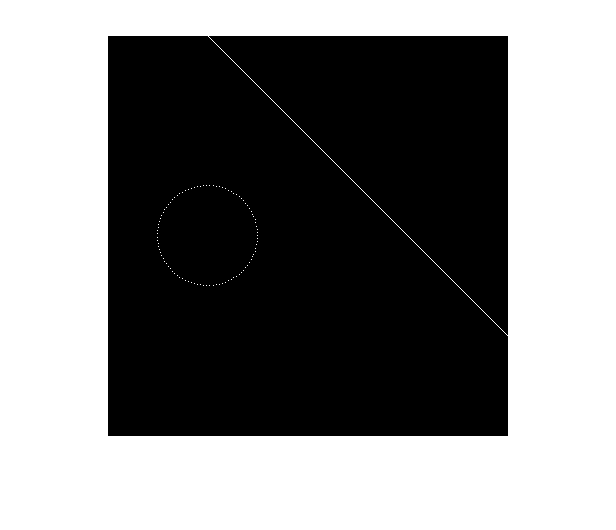
\includegraphics[width=13cm]{part2.png}
\caption{Generated binary image}
\label{fig1}
\end{center}
\end{figure}
 
\newpage
\section{Hough Transform for a Line}
Next let's try to find the parameters of that line!  Apply the \emph{Hough Transform for a Line} to your binary image.  Use the \emph{polar} form, varying the of the parameters $\theta, r$ according to the slides, and incrementing them by one for each bin.\\

\noindent
In your report, provide:
\begin{itemize}
\item The value of $(\theta, r)$ that cooresonds to the maximum value in the Hough Transform.
\item The corresponding values for $(m,b)$ where $m$ is the slope and $b$ is the y-intercept.  Show the equations/formulas that allow you to compute those from $(\theta,r)$.
\item A plot of the Hough Transform as an image.
\end{itemize}

\noindent
Your Hough Transform should look something like Figure \ref{fig2}.

\begin{figure}[H]
\begin{center}

\includegraphics[width=\textwidth, height=22cm]{part3.png}
\caption{Hough Transform for a Line}
\label{fig2}
\end{center}
\end{figure}

\newpage
\section{Hough Transform for Circle}
Next let's try to find that circle!  To find all the parameterize your circle, you'll need a 3D Hough Transform ($x_0, y_0, r$, where $x_0$ and $y_0$ are the $x$ and $y$ coordinates of the center of the circle, respectively, and $r$ is its radius).\\

\noindent
You may make the following assumptions:
\begin{itemize}
\item The circle's center is within the bounds of the image.
\item The circle's radius is less than the diagonal length of the image.
\end{itemize}

\noindent
Much like with the line, in your report, provide:
\begin{itemize}
\item The value of $(x_0, y_0, r)$ that cooresonds to the maximum value in the Hough Transform.
\item A plot of the Hough Transform as an image. \textbf{However}, since this is a 3D histogram just plot $x$ vs $y$ for the \emph{slice} where $r=rmax$ where $rmax$ is the value of $r$ find in the max bin.
\end{itemize}

\noindent
An example can be found in Figure \ref{fig3}.

\begin{figure}[H]
\begin{center}
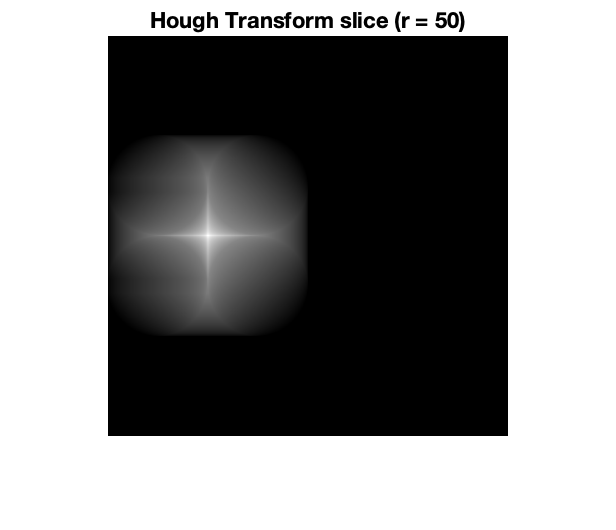
\includegraphics[width=15cm]{part4.png}
\caption{Slice of Hough Transform for a Circle}
\label{fig3}
\end{center}
\end{figure}

\newpage
\section{Apply to a Real Image}
Now let's apply this stuff to a real image!\\

\noindent
For the problem we'll use the provide image \emph{circles.gif}.  However, this is a grayscale image, not a binary image.  In your previous assigment you implemented elements of a Canny Edge Detector.  For this one you'll just use Matlab's \emph{edge} function to do this for you.  Feel free to play with any parameters of that function, but if you deviate from the defaults, put in your report what parameters you changed.\\

\noindent
Once you have your binary image, apply your Hough Circle detection to it.   Display as subplots:
\begin{itemize}
\item Original image
\item Binary image
\item Original image with dominant circle superimposed in \emph{red}.
\end{itemize}

\noindent
An example can be found in Figure \ref{fig4}.

\begin{figure}[H]
\begin{center}
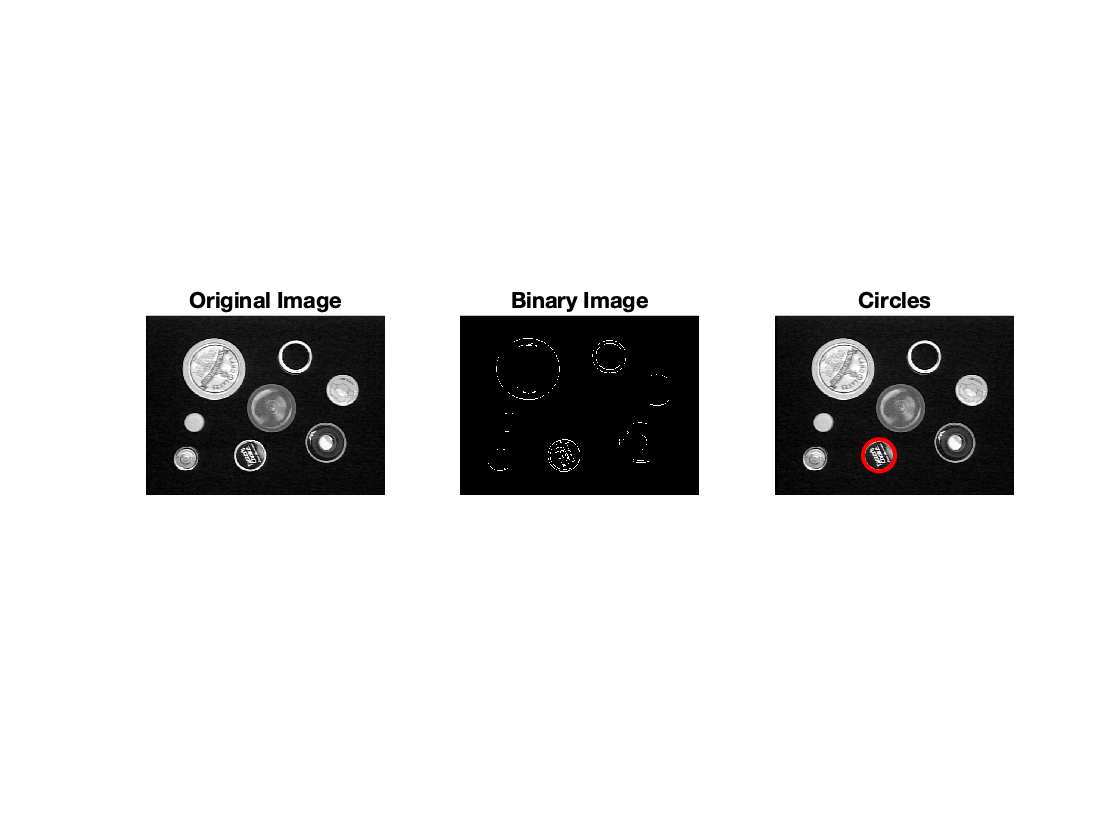
\includegraphics[width=\textwidth]{part5.png}
\caption{Circle Found!}
\label{fig4}
\end{center}
\end{figure}

\noindent
\\
In your report, provide:
\begin{itemize}
\item The value of $(x_0, y_0, r)$ that cooresonds to the maximum value in the Hough Transform.
(x0,y0,r) = (184.165188,142.681713,74.037164)
\item The subplot image described earlier.
\end{itemize}


\newpage
\section{Additional Circles}
Of course there was more than one circle in that image!  For the last part, attempt to identify all the ``major'' circles in the image.  Of course ``major'' is a bit subjective, but in general no circles should be either partial or fully enclosed in one another.  If a set are, the largest should only be kept.\\

\noindent
In your report describe how you implemented this. In addition, provide a subplot like you did in the previous part as well as the parameters of the circles you detected.  We will also test your approach on an additional image for robustness.

\begin{figure}[H]
\begin{center}
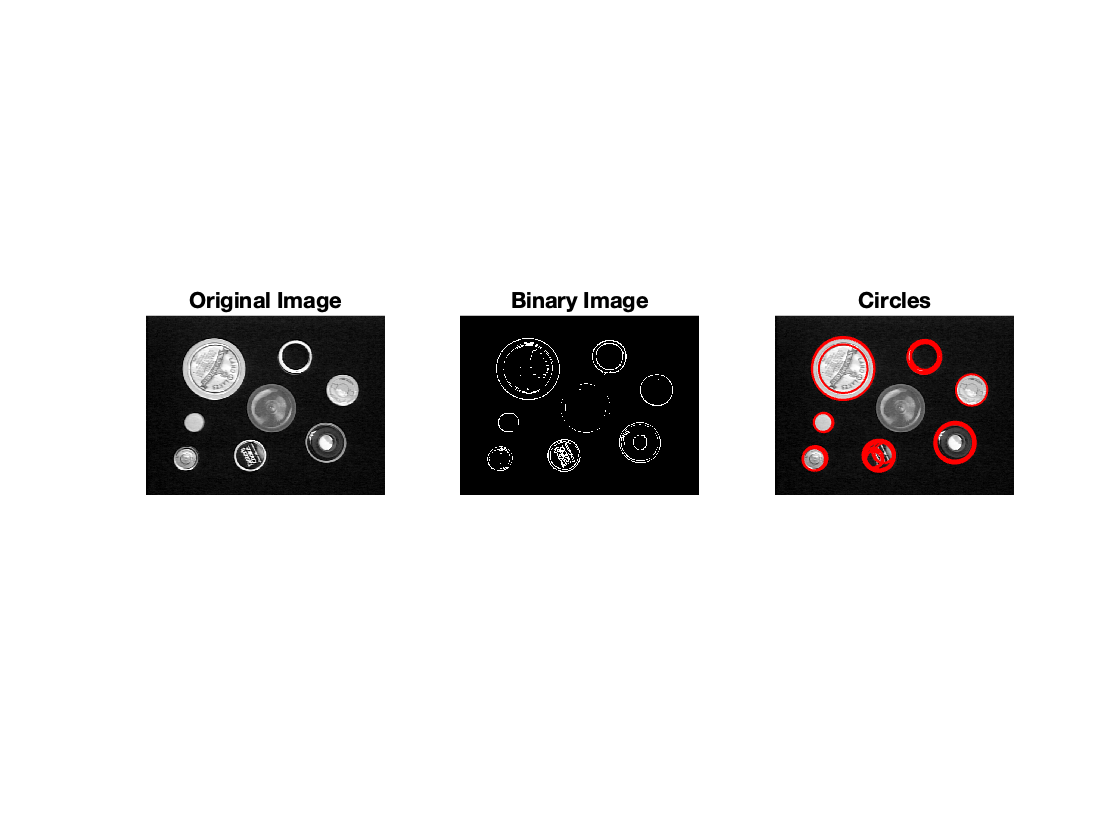
\includegraphics[width=\textwidth]{part6.png}
\caption{Circle Found!}
\label{fig4}
\end{center}
\end{figure}


Circle 1: (x0,y0,r) = (184.165188,142.681713,74.037164)\\
Circle 2: (x0,y0,r) = (336.553328,248.017919,63.597544)\\
Circle 3: (x0,y0,r) = (400.544692,109.670774,44.454298)\\
Circle 4: (x0,y0,r) = (279.307357,374.597988,42.237040)\\
Circle 5: (x0,y0,r) = (527.722224,199.456264,42.032820)\\
Circle 6: (x0,y0,r) = (108.113323,383.954081,29.525538)\\
Circle 7: (x0,y0,r) = (130.318022,285.805473,25.920350)\\


\newpage
\section*{Submission}
For your submission, upload to Blackboard a single zip file containing:

\begin{enumerate}
\item PDF writeup that includes:
\begin{enumerate}
\item Your answer to the theory question(s).
\item For Part 2, your generated binary image.
\item For Part 3, the values for $\theta$ and $r$ that provide the maximum in your Hough transform, their corresponding values for the slope and y-intercept of that line, and an image of the Hough transform.
\item For Part 4, the values for the center and radius of the circle that provides the maximum in your Hough transform as well as an image of a \emph{slice} of the Hough transform where $r$ has its maximum value.
\item For Part 5, three images:  original image, binary edge image, and original image with detected dominent circle superimposed on it.  In addition, provide the parameters of that dominant circle.
\item For Part 6, a description of your algorithm, a list of the parameters of the detected circles, the subplot image, similar to in the previous part.
\end{enumerate}
\item A README text file (\textbf{not} Word or PDF) that explains:
\begin{enumerate}
\item Any unique features of your program (if applicable).
\item Any instructions on how to run your script to reproduce your results.
\end{enumerate}
\item Your source file(s).
\end{enumerate}

\end{document}

